

\subsection{Allgemeine periodische Anregung}

\begin{frame}
\frametitle{Superpositionsprinzip}
\begin{center}
\begin{tikzpicture}
\draw (0, 0.21) node {Lineares};
\draw (0,-0.21) node {System};
\draw (-1,-0.5) rectangle (1, 0.5);
\draw[->] (-4, 0) -- (-1, 0);
\draw[->] ( 1, 0) -- ( 4, 0);
\draw[visible on=<1>] (-2.5, 0.25) node {$a_1(t)$};
\draw[visible on=<1>] ( 2.5, 0.25) node {$u_1(t)$};
\draw[visible on=<2>] (-2.5, 0.25) node {$a_2(t)$};
\draw[visible on=<2>] ( 2.5, 0.25) node {$u_2(t)$};
\draw[visible on=<3->] (-2.5, 0.25) node {$a_1(t)+a_2(t)$};
\draw[visible on=<3->] ( 2.5, 0.25) node {$u_1(t)+u_2(t)$};
\end{tikzpicture}

\end{center}
\uncover<3>{
Vorgehen für den (allgemein) periodisch erregten Einmassenschwinger 
\begin{align*}
a(t)&=\frac{1}{2}A_0 + \sum_{k=1}^{\infty} A_k \cos\left(\frac{2\pi kt}{T}\right) + B_k\left(\frac{2\pi kt}{T}\right)\\
&\approx\frac{1}{2}A_0 + \sum_{k=1}^{N} A_k \cos\left(\frac{2\pi kt}{T}\right) + B_k\left(\frac{2\pi kt}{T}\right)\\
u(t)&= \sum_{k=1}^{\infty} u_k(t) \approx \sum_{k=1}^{N} u_k(t)
\end{align*}
}
\end{frame}


\begin{frame}
\frametitle{Anwendungsbeispiel}
\begin{figure}
 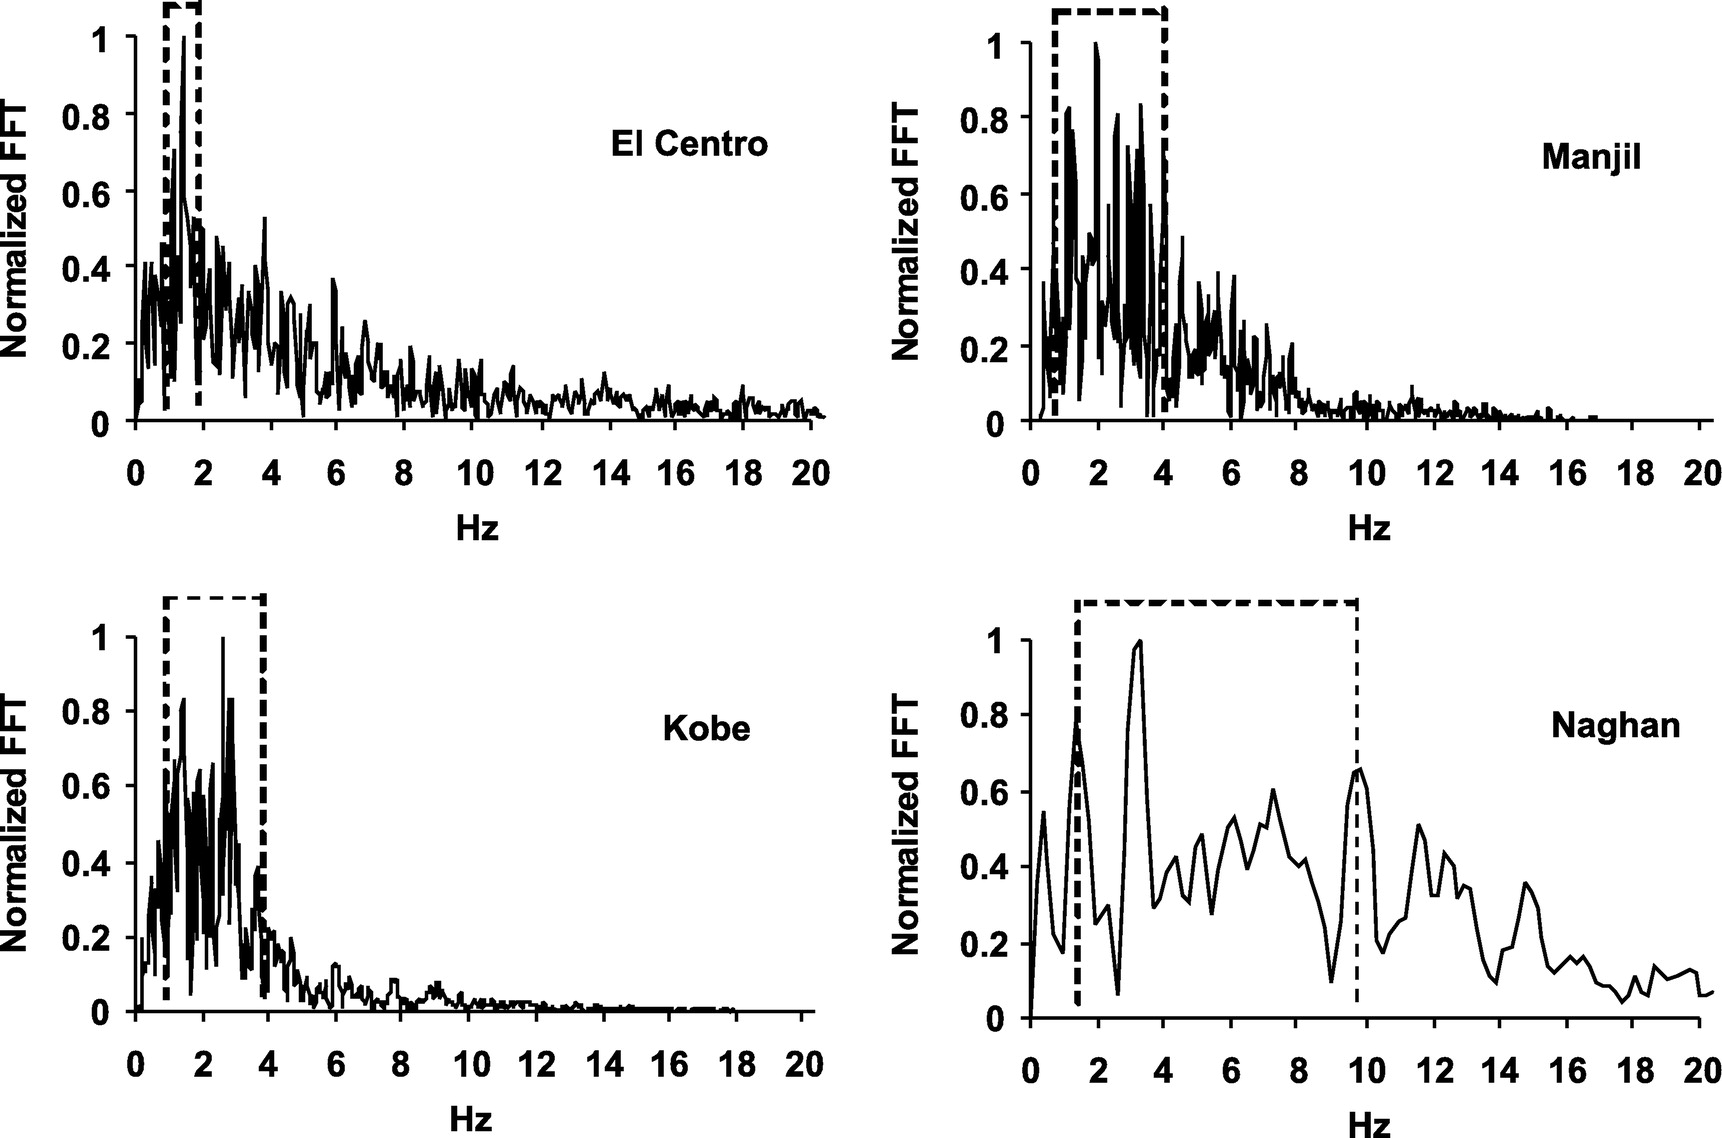
\includegraphics[width=0.7\textwidth]{fig_img/earthquake_spectra.jpg}
 \caption*{Amplitudenspektrum ausgewählter Erdbeben \cite{amiri2008}}
\end{figure}
Anmerkung: Dieses Vorgehen wäre für Überschlagsrechnungen angebracht.

\end{frame}



\begin{frame}
\frametitle{Zusatzmaterial} % physical intution and complex representation
\vfill
\begin{center}

\includegraphics[width=0.2\textwidth]{fig_img/youtube.png}  

\href{https://www.youtube.com/watch?v=spUNpyF58BY}{\textsl{3Blue1Brown: Was ist eine Fourier-Transformation?}}
\end{center}  
\vfill
\end{frame}
